\documentclass{article}

\usepackage{amsmath}
\usepackage{amssymb}
\usepackage{graphicx}

\begin{document}


Ivan Lin\newline{}
Dr. Esther Arkin\newline{}
AMS301\newline{}
1/25/17

\begin{center}
  Homework 1a
\end{center}

\underline{Section 1.1 Problem 2}

a. Directed graph indicating a team beat another team:

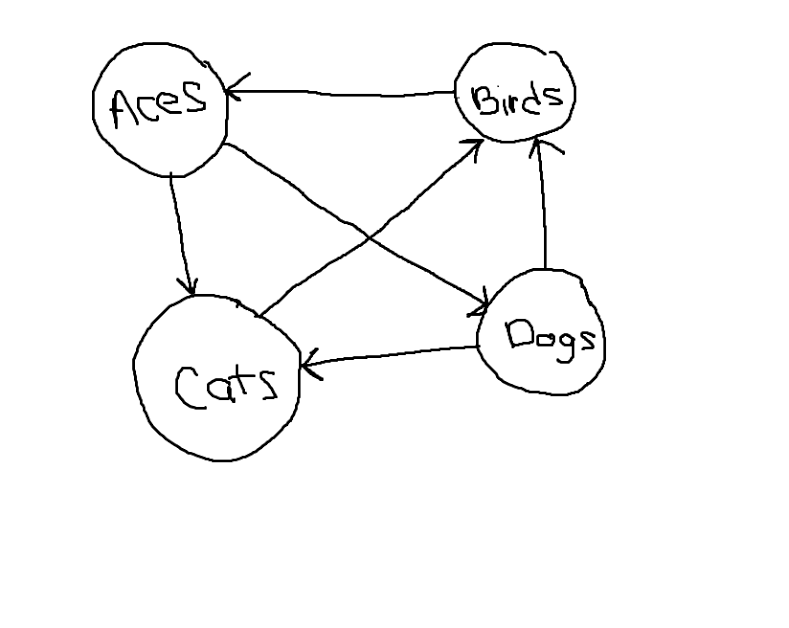
\includegraphics[width=\textwidth]{2a.png}\newline{}

b. Dominance orders:
\begin{itemize}
\item Aces, Dogs, Cats, Birds
\item Birds, Aces, Dogs, Cats
\item Cats, Birds, Aces, Dogs
\item Dogs, Birds, Aces, Cats
\item Dogs, Cats, Birds, Aces\newline{}
\end{itemize}


\underline{Section 1.1 Problem 24}

The largest independent set in a circuit of length 7 is of size 3.\newline{}
To maximize the size of the independent set, there should only be one vertex between every member of the set, which means three vertices would form an independent set and the four remaining vertices would separate the three so they are not adjacent.\newline{}
The largest independent set in a circuit of length $n$ is of size $\frac{n}{2}$ if $n$ is even and size $\frac{n-1}{2}$ if $n$ is odd. Alternatively the answer is $floor(n)$.\newline{}
This is by the same reasoning as above. For every vertex in an independent set, there must be at least one not in the set to separate it from other vertices in the set.\newline{}


\underline{Supplement II Problem 5}

Show that at least two vertices have the same degree in any graph with at least
two vertices.

\textit{Proof}

We will prove by contradiction that graphs with more than two vertices have at least two vertices with the same degree.

Assume for the sake of contradiction that in a graph with $n$ vertices where $n \geq 2$, each vertex has a different degree.

Any vertex in the graph can't have a degree higher than $n-1$, since there are only $n-1$ other vertices to which it can be connected without parallel connections or self loops.

This means there is a 1-to-1 mapping of vertices to distinct degree values, where the $1st$ vertex has a degree of $0$ and the $i-th$ vertex has a degree of $i-1$. 

This means that the $n-th$ vertex has a degree of $n-1$. However, since the first vertex has a degree of $0$, there are only $n-2$ other vertices to which the $n-th$ vertex could be adjacent.

Therefore we have proven by contradiction that graphs with more than two vertices must have at least two vertices with the same degree.\newline{}

\underline{Supplement II Problem 6}

Show that an undirected graph with all vertices of degree $\geq 2$ must contain a circuit (edges cannot be repeated in a circuit).

\textit{Proof}

We will prove that a graph with all vertices of degree $\geq 2$ must contain a circuit.

Let $i$ denote a vertex in a graph with $n$ vertices.

For the first vertex, $i=1$, let vertices $i+1, i+2, ...$ represent the vertices to which it is adjacent.

All other vertices $i>1$ must have at least one other adjacent vertex denoted by a value $\geq i$, since all previous numbers have a path to the first vertex and therefore each other.

However, for $i=n$, there exists no other eligible vertex. There already exists a path to every other vertex, so any valid edge would form a circuit.

We have proven that graphs with all vertices of degree $\geq 2$ must have a circuit.
\end{document}
